% This section provides a high-level statement of your product concept - what it is intended to do and how it is intended to be used. Include in this header paragraph, a brief synopsis of what is described here. For example, this header paragraph might say something like: "This section describes the purpose, use and intended user audience for the X product. X is a system that performs Y. Users of X will be able to Z..."

This section describes the purpose, use \& intended audience for our programmed UR5 collaborative robot (co-bot). The UR5 co-bot will be programmed to be able to play the interactive \& strategy-based game, checkers, against a human opponent. The robot will have an electropermanent magnetic attachment that will allow it to pick up and move the individual checkers pieces. The robot is not intended to beat the human opponent every time but rather just have the ability to play a full game of checkers against them.

\subsection{Purpose and Use}
% This is where you describe in a brief, yet clear and concise, manner what your product should do and how you expect it should be used.

Our project aims to showcase the UR5 co-bot's abilities as a means of promoting the UT Arlington College of Engineering to prospective students through the means of an interactive demonstration. Students visiting the College of Engineering are expected to be able to engage with the product in a game of checkers, which will provide the potential Mavericks with an enjoyable and educational experience.

\subsection{Intended Audience}
% This is where you describe the intended audience(s) of your product. If this product were to be made available publicly or commercially, who would purchase or use it? Is the product designed for a particular customer, or an overall class of customers? Is it intended for general use, or is it a specific component of a more complex system?

The intended audience of our product is the UT Arlington College of Engineering, Department of Computer Science \& Engineering as well as the university as a whole to utilize the co-bot as a marketing strategy for prospective students. If this product were to be made commercially available it would be feasible and our primary customers would be other universities aiming to also recruit future engineers. Although the UR5 co-bot is intended to be operated by a student or faculty member of the university, the end user is a member of the public as the project is intended for general use.

\begin{figure}[h!]
	\centering
   	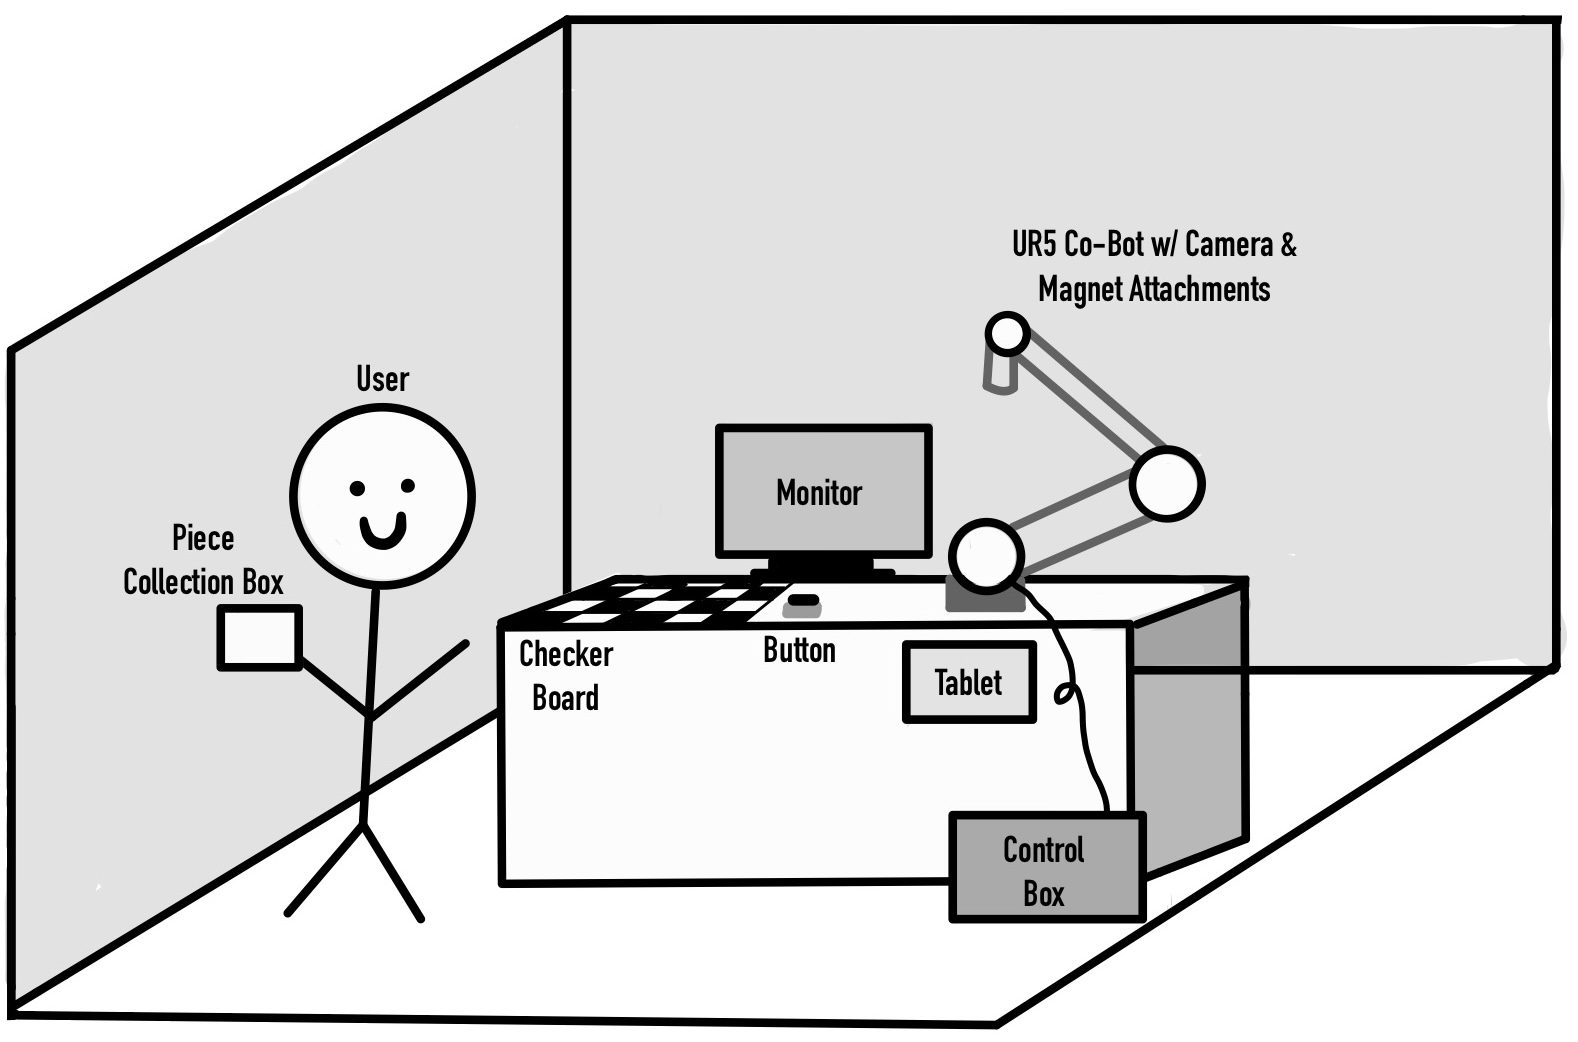
\includegraphics[width=0.90\textwidth]{images/Conceptual-Drawing.jpg}
    \caption{Conceptual Drawing}
\end{figure}
